\documentclass[sigconf]{acmart}
\AtBeginDocument{%
  \providecommand\BibTeX{{%
    \normalfont B\kern-0.5em{\scshape i\kern-0.25em b}\kern-0.8em\TeX}}}
    
\usepackage{amssymb}
\usepackage{amsmath}
\usepackage{pgfplots}
\usepackage{svg}
\usepackage{booktabs}% http://ctan.org/pkg/booktabs
\usepackage{tikz}
\usepackage{listings}
\usepackage{multirow}% http://ctan.org/pkg/multirow
\pgfplotsset{width=10cm,compat=1.9}

\begin{document}

\title{Smart-Cache: Pre-fetching Using Markov Chains in Distributed Caching}

\author{Meia Alsup}
\authornote{Denotes equal contribution.}

\affiliation{%
  \institution{Massachusetts Institute of Technology}
  \streetaddress{77 Massachusetts Avenue}
  \city{Cambridge}
  \state{MA}
}
\author{Amir Farhat}
\authornotemark[1]
\affiliation{%
  \institution{Massachusetts Institute of Technology}
  \streetaddress{77 Massachusetts Avenue}
  \city{Cambridge}
  \state{MA}
}
\author{Alexander J. Root}
\authornotemark[1]
\affiliation{%
  \institution{Massachusetts Institute of Technology}
  \streetaddress{77 Massachusetts Avenue}
  \city{Cambridge}
  \state{MA}
}

\renewcommand{\shortauthors}{Alsup*, Farhat*, Root*}

\begin{abstract}
Current caching methods for distributed data-stores do not detect patterns in data accesses. Many types of data accesses, such as web page accesses and machine learning workloads have simple patterns that can be detected via a Hidden Markov Model (HMM). This work presents Smart-Cache, a distributed caching model that uses HMMs to predict future data accesses and prefetch data according to some learned patterns. We have implemented this cache and compared it to a \texttt{memcached}-like cache that does no data prefetching. Smart-Cache provides significant speed up on workloads with patterns. The experiments conducted show execution time reduction of 23\% for deterministic workloads and 8\% for lightly patterned workloads.

\end{abstract}

\keywords{distributed systems, caching, markov chain, distributed learning}

\maketitle

\section{Introduction and Related Work}
\label{sec:intro}

Efficient, distributed caching is a well-known solution to alleviating load on underlying and expensive-to-query data stores \cite{Memcached}. Some caching systems attempt to predict future data accesses and pre-fetch accordingly.  Previous efforts to optimize pre-fetch mechanisms have relied on assumptions around data locality \cite{SequentialPrefetch}; few methods relax the locality assumption for truly un-opinionated cache pre-fetch prediction. 

Memcached also uses Consistent Hashing to distribute load across caches \cite{ConsistentHash}. Consistent Hashing is complex and makes Memcached resilient to hot files, and dynamically reallocates responsibility for files amongst caches in a cache-locality aware way. Smart-Cache takes a much simpler approach to distribution of file responsibility amongst caches, which greatly reduces the overhead while still providing good performance.

Markov chains have been shown to learn data access patterns in many other settings including file I/O, hard disks access, and in smaller scale buffers or pages \cite{Lynx, MarkovPredictors, TaP}. Smart-cache is motivated in particular by the deep learning workload scenario, but is generalizable and usable by a much wider array of scenarios with patterned workload accesses.

Machine leaning workloads, which are traditionally bottlenecked by compute power and GPU cycles, benefit from new hardware so as to put increasing load on underlying datastores. With state-of-the-art hardware, these datastores become a significant bottleneck \cite{kahn2020scaling}. In such situations, even a simple caching layer in front of the datastore gives huge reductions in datastore egress requirements and significantly lowers round-trip request latency \cite{kahn2020scaling}. When training large deep neural networks, most hyper paramter optimization procedures require that a large set of training runs are started, each with different hyper-paramater configurations. While each run has a different configuration, all runs access data in the same order. These runs, which are often in the same cluster of GPUs, all make queries to data with the same access pattern.

Our contributions are three fold. First, we introduce Smart-Cache, a fault-tolerant and distributed cache based on memcached \cite{fitzpatrick2004distributed} that can dynamically learn data access patterns. Second, we provide a simple patterned workload generator to proxy web workloads. Third, we characterize the performance of Smart-Cache on three workloads with varying degrees of contained patterns, and demonstrate significant improvement with respect to both latency measurements and queries to the underlying datastore.

\section{System and Setup}
\label{sec:system}


\subsection{Design}
\label{sec:design}
\subsubsection{Assumptions}
\label{sec:assumptions}

We assume a static underlying datastore. Smart-Cache takes initial inspiration from machine learning workloads. ML workloads are short-lived on a static underlying dataset, where modifications to the underlying datastore only occur between task runs. In the first iteration of Smart-Cache, a static underlying datastore is assumed, which enables a simple design.

We also assume similar file popularity amongst files in the datastore. This version of Smart-Cache is not resilient to hot files and nodes.

Extensions to Smart-Cache to mitigate the effects of both of these assumptions are discussed in Section \ref{sec:conclusion}.

\subsubsection{System Design}
\label{sec:systemdesign}

\begin{figure}[h]
  \centering
  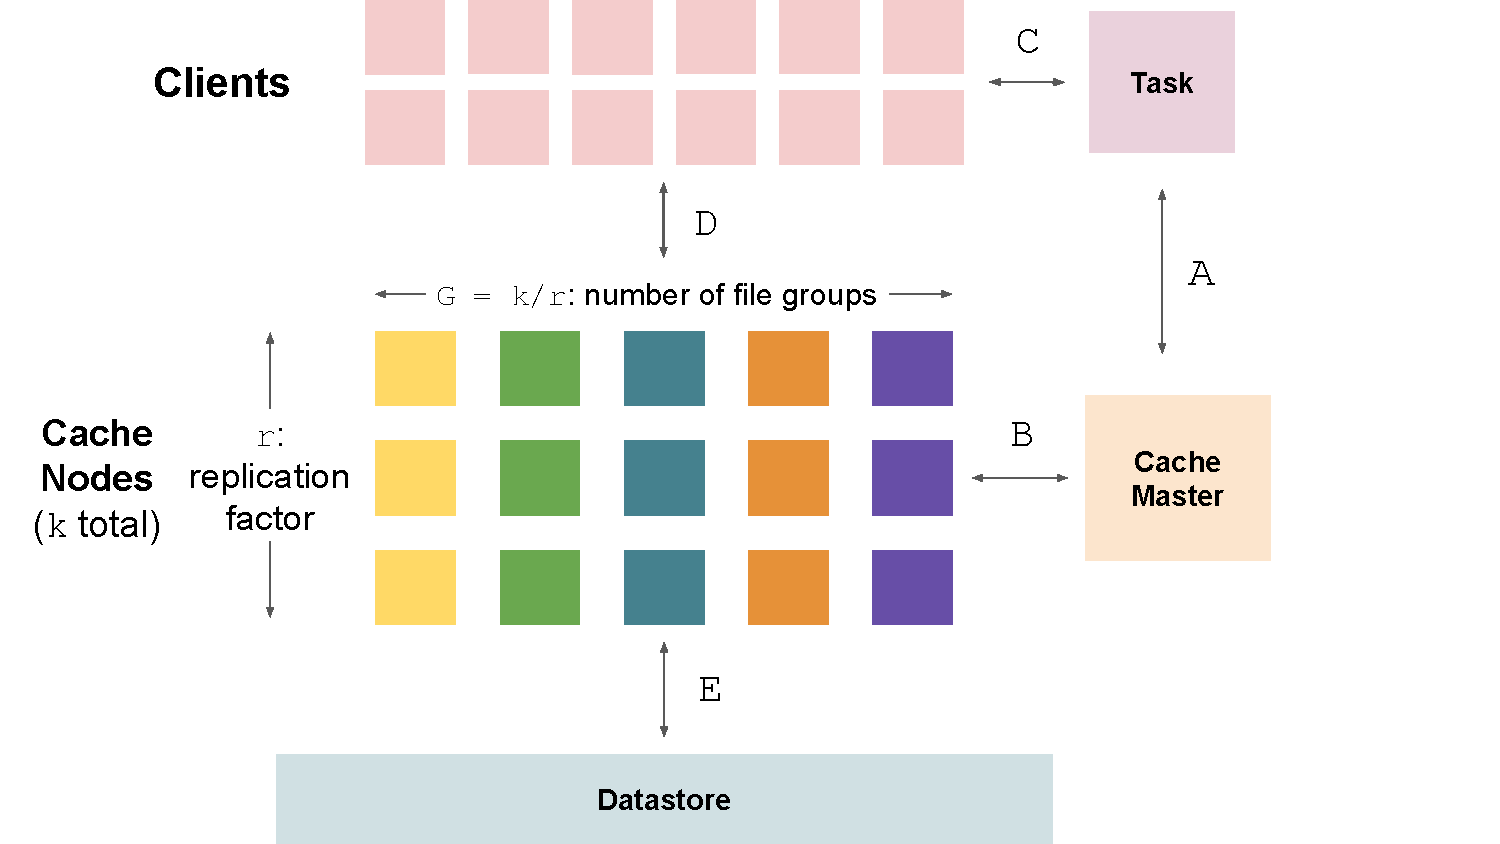
\includegraphics[width=\linewidth]{systemdiagram.pdf}
  \caption{\label{fig:systemdesign} Smart-Cache System Diagram. Communication channels (labeled A, B, C, D, E) are discussed in \ref{sec:execution}. }
  \Description{Smart-Cache System Diagram}
\end{figure}

Figure \ref{fig:systemdesign} shows the system components. Smart-Cache supports a single task at a time, which coordinates many clients. The task interacts with \textit{Cache master} which coordinates the behavior of the individual caching nodes. \textit{Caching nodes} cache and store data, and are the only nodes connected to the underlying datastore. 


The number of cache nodes, $k$, and the replication factor $r$, are configurable. These two parameters determine the number of file groups, $G=\frac{k}{r}$. In the event $r$ is not divisible by $k$, the floor is used and extra caches are allocated to file groups at random. These parameters allow the user to scale the caches along two axes. In Figure 1, $k$ is $15$, $r$ is $3$, and the number of file groups $G$ is $5$. File groups are color coded. The cache master (CM) handles distributing files across the $G$ file groups. Consider the underlying data-set $\mathcal{D}$ and $\{d_1, ..., d_g\}$ as disjoint subsets of $\mathcal{D}$ such that $\mathcal{D} = \bigcup_{i = 1}^n d_i$. For each subset of $d_i \subseteq \mathcal{D}$, a file group is responsible for that subset and the subset is replicated across $r$ caching nodes. 


CM assigns subsets $D_i$ to each file group. CM also dictates which caches a client fetches data from. CM creates a hash function, as described in Section \ref{sec:hash}, in order to create a mapping from a client ID and filename to an ordering on the cache IDs in the relevant file group. This mapping handles spreading the load for files in a file group across the replicated caches in that group. Each client gets back a list of all the cache IDs in the file group of interest. This is the order the client tries to fetch the file in. On failure, the client will try the fetch from the next cache ID.

\subsubsection{Execution Flow and Communication}
\label{sec:execution}

A task is initiated with a call to CM over Channel A in \ref{fig:systemdesign}. The task tells CM the client IDs, the files in the datastore, and the configuration parameters for the cache. The cache master spins up cache nodes, and assigns each cache responsibility for a subset of the datastore - this happens over Channel B. The cache nodes are responsible for fetching files from the datastore over Channel E. CM shares the mapping function from client IDs and files to cache lists with the task over channel A, which distributes this information to each client over channel C. The clients \textit{do not directly interact with the cache master nor datastore}, but instead utilize the mapping to go fetch files from the correct cache nodes over Channel D. 

\subsubsection{Fault Tolerance}
\label{sec:faulttolerance}

Increasing $r$ facilitates better redundancy as more caching nodes tasked with caching files from $d_i$ can fail before the system is unable to serve assets from $d_i$. While our implementation doesn't do so, nodes serving data from another subset of $\mathcal{D}$ can be re-purposed to serve files from $d_i$ if enough nodes fail such that the number of nodes serving data from each subset remains balanced.


While we assume that the load on each subset of $\mathcal{D}$ is uniform, the number of nodes serving a particular subset can also be modified to balance the load placed on that subset by clients. As such, the replication factor for each subset may not be uniform, but can be proportional to the required load.


This setup provides fault-tolerance configurable to the user, through the replication parameter. Without the optimizations to re-balance caches mentioned above, if all caches fail in a given file group, the whole task fails. This is an acceptable trade-off as replication is configurable and the probability that all caches in a file group fail concurrently 


\subsection{Experiments and Workload Types}

Our experimental setup consists of a \textit{task} for a given workload type, which is run on an instance of Smart-Cache. The task spins up several clients, each of which must complete the workload assigned by the task. 

Our terminology follows: 
\begin{itemize}
\item \textit{Task}: Over-arching "workload master". which starts many clients each of which have their own workload. 
\item \textit{Client}: A machine spun up by the task. The client is responsible for a single workload, which is assigned by the task. This workload specifies the order in which the client will request the files from the caching layer.
\item \textit{Workload}: This term is overloaded. In the context of a client, "workload" refers to file access order assigned to the client by the task. More generally, "workload" refers to a generic type that the file access order represents - i.e., Deterministic (Machine Learning), Patterned (Web), or Random.
\end{itemize}

We analyze three workload types (these are defined in \ref{subsubsection:workloads}). For each workload we run the task to completion twice, once using Smart-Cache with Markov based pre-fetching, and once without pre-fetch. The no-prefetch scenario is used to benchmark the performance improvement attributable to the Markov chain based approach. In total we ran 6 tasks, the cross product between our three workload types with the two prefetch mechanisms: no prefetch and Markov chain based prefetch.

 
\subsubsection{Workload Types}
\label{subsubsection:workloads}
\begin{itemize}
    \item \textbf{Deterministic}: The task gives all clients the same workload. Each client has the exact same file access pattern. Machine learning workloads are an example of a deterministic workload.

     \item \textbf{Patterned}: Patterned workloads share some patterns in data accesses across client workloads. The expectation is that all clients exhibit similar behavior, but not exactly the same. The methodology used to generate patterned workloads is explained in \ref{sec:patternedworkloads} 
     These patterned workloads are not drawn from any scenario in particular. However, web workloads are an example of a patterned workload. Web traffic is characterizes by popular page transitions. Therefore, a pattern can represent a transition from web page 1 to web page 2 that is common. Further, a given web-page often loads content using multiple rounds of requests. Every client that loads this page will make the same synchronous requests to fill the page, which accesses the underlying datastore in the same order every time.
    
    \item \textbf{Random}: Random workloads exhibit no patterns. The workloads for each client are generated randomly and completely independently. The random workload is important to benchmark the improvements seen in Deterministic and Patterned workloads, as well as to understand if Smart-Cache slows down performance in the case there is no pattern to learn.
\end{itemize}

Our workload generator can be found in our released code, see Section \ref{sec:code}.


\subsection{Markov Prefetching Model}
\label{sec:markovchain}
Each cache stores a model of file access patterns for the particular cache. We use a sparse Markov model \cite{xiong2016SparseMarkov}, as it is expected that a series of accesses with commonly occurring patterns is best represented in a sparse model. Assuming constant degree $d_i$ for each of the $n$ nodes, $i \in [0, n)$, then a sparse representation takes $\Theta(n)$ memory as opposed to a dense model that requires $\Theta(n^2)$ memory. 

Using this model, we can implement an efficient predictor that takes a source file and can predict the next $k$ file accesses in $\Theta(k \log(k))$ time, using a modification of Dijkstra's algorithm \cite{dijkstra1959}. The problem formulation involves a reduction from an attempt to maximize the product of probabilities in the range $(0, 1]$ to a maximization of the logarithm of the product, which reduces to a minimization of the sum of the logarithm of the probabilities, which reduces to a formulation of Dijkstra's, as the edge weights are strictly non-negative. It is important to not that this algorithm is aggressively sublinear, as the predictor does not depend on the number of files $n$ that a given cache is responsible for.



\section{Results}
\label{sec:results}
The results from our runs in time are shown in Table \ref{tab:freq}. Hits and misses to the underlying datastore for each of our runs are shown in Table \ref{tab:hits}.

A limitation of the results is that these workloads were run locally on our machines, instead of on a dedicated compute cluster. These results are also for a single run rather than an average across several runs. As such, the difference observed in the Random task between LRU and Markov Chain is likely not statistically significant. However, the result on the Deterministic task is likely significant.

\begin{table}[h]
  \caption{Total time in seconds to perform tasks.}
  \label{tab:freq}
  \begin{tabular}{ccl}
    \toprule
     & LRU  & Markov Chain \\
    \midrule
 Random & 11.11 & 19.12 \\
 Patterned  & 30.01 & 27.46 \\
 Deterministic  & 26.53 & 20.47 \\
  \bottomrule
\end{tabular}
\end{table}


\begin{table}[h]
  \caption{ Hits and Misses}
  \label{tab:hits}

    \begin{tabular}{c@{\qquad}ccc@{\qquad}ccc}
      \toprule
      \multirow{2}{*}{\raisebox{-\heavyrulewidth}{Workload Type}} & \multicolumn{2}{c}{LRU} & \multicolumn{2}{c}{Markov Chain} \\
      \cmidrule{2-5}
      & Hits & Misses  & Hits & Misses \\
      \midrule
      Random & 404 & 2596  & 400 & 2600  \\
      Patterned & 1112 & 1062 & 1638 & 536  \\
      Deterministic & 9000 & 1000 & 9898 & 102  \\
      \bottomrule
    \end{tabular}

\end{table}

\begin{figure}[h]
    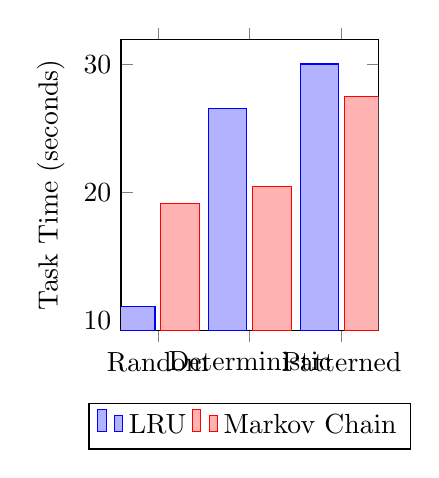
\begin{tikzpicture}
    \begin{axis}[
        ybar,
        width=\textwidth / 2.5,
        height=150,
        enlarge x limits={0.2},
        /pgf/bar width=14pt,% bar width
        legend style={at={(0.5,-0.25)},
          anchor=north,legend columns=-1},
        ylabel={Task Time (seconds)},
        symbolic x coords={Random,Deterministic,Patterned},
        xtick=data,
    ]
    
    % LRU
    \addplot coordinates {(Random,11.11) (Deterministic,26.53) (Patterned,30.01)};
    % Markov Chain
    \addplot coordinates {(Random,19.12) (Deterministic,20.47) (Patterned,27.46)};
    \legend{LRU, Markov Chain}
    \end{axis}
    \end{tikzpicture}
    \caption{\label{fig:test_times}Total time to perform tasks, in seconds, across workloads and caching strategies.}
\end{figure}

\begin{figure}[h]
    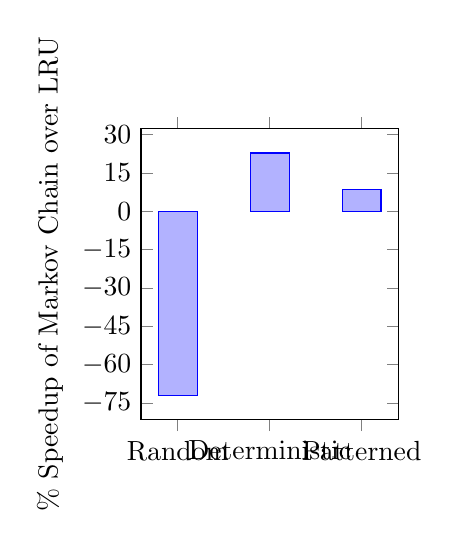
\begin{tikzpicture}
    \begin{axis}[
        ybar,
        width=\textwidth / 2.5,
        height=150,
        enlarge x limits={0.2},
        /pgf/bar width=14pt,% bar width
        legend style={at={(0.5,-0.25)},
          anchor=north,legend columns=-1},
        ylabel={\% Speedup of Markov Chain over LRU},
        symbolic x coords={Random,Deterministic,Patterned},
        xtick=data,
        ytick distance=15
    ]
    
    % Markov Chain
    \addplot coordinates {(Random,-72) (Deterministic,22.8) (Patterned,8.5)};
    \end{axis}
    \end{tikzpicture}
    \caption{\label{fig:test_times} \% speedup to perform tasks between caching strategies for each workload}
\end{figure}


\section{Conclusion and Future Work}
\label{sec:conclusion}
In this paper, we demonstrate the utility of Smart-Cache to speed up workloads that exhibit patterns. This is immediately useful for machine learning applications and in any other application where workloads can be characterized by repeat data access patterns. 

This can be expanded upon on a few axes. The cache master can dynamically allocate cache nodes across file groups to prevent hot files from taking the system down and make the system more resilient to caches going down in a particular file group. The system currently uses a simple hashing scheme, but more complex hashing schemes such as consistent hashing \cite{ConsistentHash} can be leveraged to make the system more tolerant to caches going off and online.

Further, the cache master could implement periodic Markov chain syncing across caches in the same file group. This would enable learning to happen quicker, since patterns observed can be learned at double or triple the speed for a replication factor of two or three respectively. 

Another extension to Smart-Cache is supporting a dynamic underlying datastore. This requires the cache-master to allocate and de-allocate files as they are added and deleted from the datastore. With respect to staleness, a system leveraging version numbers could be used, or writes could be set up to notify all caches in the affected file group that the data is stale and in need of refresh.




\begin{acks}
We'd like to thank Professor Robert Morris, Anish Athalye, and the entire 6.824 staff for guidance and helpful conversations. We would also like to thank Jacob Kahn for providing insight into machine learning workloads at Facebook AI Research, and inspiring this work.
\end{acks}


\appendix
\section{Appendix}
\label{sec:appendix}

\subsection{Code}
\label{sec:code}
Our released codebase for Smart-Cache as well as task and workload generation can be found on our Github: \url{https://github.com/rootjalex/smart-cache}.

\subsection{Patterned Workloads}
\label{sec:patternedworkloads}

Patterned workloads are generated by first creating short access patterns that will be common amongst clients. In our test runs, we generate 10-200 patterns, depending on the benchmark. From this set of patterns, the workload for each client is created by randomly sampling a pattern from the pattern set 2-10 times, and concatenating them. 


To make this concrete, the following example illustrates a potential outcome with two patterns and two client workloads each composed of five randomly concatenated patterns.
\begin{itemize}
    \item The two randomly generated patterns are {\fontfamily{qcr}\selectfont[A.txt,
    
    B.txt, C.txt]} and {\fontfamily{qcr}\selectfont[X.txt, Y.txt]}.
    \item Client 1 has workload: {\fontfamily{qcr}\selectfont[A.txt, B.txt, C.txt, 
    
    A.txt, B.txt, C.txt, A.txt, B.txt, C.txt, X.txt, Y.txt, X.txt, Y.txt]}
    \item Client 2 has workload: {\fontfamily{qcr}\selectfont[X.txt, Y.txt,
    A.txt,
    
    B.txt, C.txt, X.txt, Y.txt, X.txt, 
    
    Y.txt, A.txt, B.txt, C.txt]}
\end{itemize}

\subsection{Cache Responsibility - Hashing Function}
\label{sec:hash}

The hash function generator takes the following inputs: number of caches ($k$), cache replication factor ($r$), list of client IDs, and filenames ($n$ files total) in the  underlying datastore. The following steps generate the hash function:
\begin{enumerate}
\item The number of file groups, $G$, is determined from $\frac{k}{r}$. Caches are allocated evenly across file groups such that each group is responsible for [$r$, $r+1$] caches in the event of overflow.
\item Responsibility for the $n$ files is divided across the $G$ file groups evenly such that each file group is responsible for [$\lfloor\frac{n}{G}\rfloor$, $\lfloor\frac{n}{G}\rfloor +1$] files. Responsibility is split randomly leveraging Go's Random package \footnote{https://golang.org/pkg/math/rand/}.
\item A mapping is created from (client ID, filegroup) $\rightarrow$ [list of cache IDs] for all pairs of client IDs and file names. For every file group and for every client ID, the list of cache IDs assigned to that file group is shuffled randomly. The ordering determined here is the order the client will attempt to retrieve files from caches. This random shuffling helps ensure that no one cache in any file group is fielding too many requests at once. A round robin method was also considered. However, with round robin, if one cache goes down, the cache immediately downstream becomes responsible for twice as many clients. Shuffling mitigates this problem since clients assigned to a dead cache redistribute amongst the remaining alive caches at random. While this is not necessarily exactly an even split, in a large system with many caches and clients, the split is expected to be almost even and sufficient.
\end{enumerate}


\bibliographystyle{ACM-Reference-Format}
\bibliography{bibliography}

\end{document}

\endinput


